%%%%%%%%%%%%%%%%%%%%%%%%%%%%%%%%%%%%%%%%%
% Thin Sectioned Essay
% LaTeX Template
% Version 1.0 (3/8/13)
%
% This template has been downloaded from:
% http://www.LaTeXTemplates.com
%
% Original Author:
% Nicolas Diaz (nsdiaz@uc.cl) with extensive modifications by:
% Vel (vel@latextemplates.com)
%
% License:
% CC BY-NC-SA 3.0 (http://creativecommons.org/licenses/by-nc-sa/3.0/)
%
%%%%%%%%%%%%%%%%%%%%%%%%%%%%%%%%%%%%%%%%%

%----------------------------------------------------------------------------------------
%	PACKAGES AND OTHER DOCUMENT CONFIGURATIONS
%----------------------------------------------------------------------------------------

\documentclass[a4paper, 11pt]{article} % Font size (can be 10pt, 11pt or 12pt) and paper size (remove a4paper for US letter paper)

\usepackage[protrusion=true,expansion=true]{microtype}	% Better typography
\usepackage{graphicx} 		% Required for including pictures
\usepackage{wrapfig}  		% Allows in-line images
\usepackage{hyperref}		% Allows the use of hyperlinks
\usepackage{amsmath}
\usepackage{multirow}
\usepackage{rotating}
\usepackage{makecell}
\usepackage{diagbox}

\usepackage{mathpazo}		% Use the Palatino font
\usepackage[T1]{fontenc} 	% Required for accented characters
\usepackage[utf8]{inputenc}     % Spanish characters
\usepackage{amsmath} 		% Allows align
\usepackage{listings}		% Allows code 
\usepackage{float}		% Allows code 
\usepackage{subfig}


\lstset{basicstyle=\footnotesize\ttfamily,breaklines=true}

\linespread{1.05} % Change line spacing here, Palatino benefits from a slight increase by default

\makeatletter
\renewcommand\@biblabel[1]{\textbf{#1.}} % Change the square brackets for each bibliography item from '[1]' to '1.'
\renewcommand{\@listI}{\itemsep=0pt} % Reduce the space between items in the itemize and enumerate environments and the bibliography

\renewcommand{\maketitle}{ % Customize the title - do not edit title and author name here, see the TITLE block below
\begin{flushright} % Right align
{\LARGE\@title} % Increase the font size of the title

\vspace{50pt} % Some vertical space between the title and author name

{\large\@author} % Author name
\\\@date % Date

\vspace{40pt} % Some vertical space between the author block and abstract
\end{flushright}
}

%----------------------------------------------------------------------------------------
%	TITLE
%----------------------------------------------------------------------------------------

\title{\textbf{Redes Neuronales Artificiales}}

\author{
	\textsc{Agustín Mista}\\
	\textit{Universidad Nacional de Rosario}\\
 	\textit{Introducción a la Inteligencia Artificial}
}

\date{Rosario, 24 de Mayo de 2017}

%----------------------------------------------------------------------------------------

\begin{document}

\maketitle % Print the title section

%----------------------------------------------------------------------------------------
%	ABSTRACT
%----------------------------------------------------------------------------------------

%\renewcommand{\abstractname}{Summary} % Uncomment to change the name of the abstract to something else

%\begin{abstract}
%	Cuando todo esté cocinado, voy a completar este abstract con información pertinente.
%\end{abstract}

\vspace{20pt} % Some vertical space between the abstract and first section

%----------------------------------------------------------------------------------------
%	ESSAY BODY
%----------------------------------------------------------------------------------------

\section*{Introducción}

\begin{wrapfigure}{o}{0.45\textwidth}
	\begin{center}
		\vspace{-20pt}
		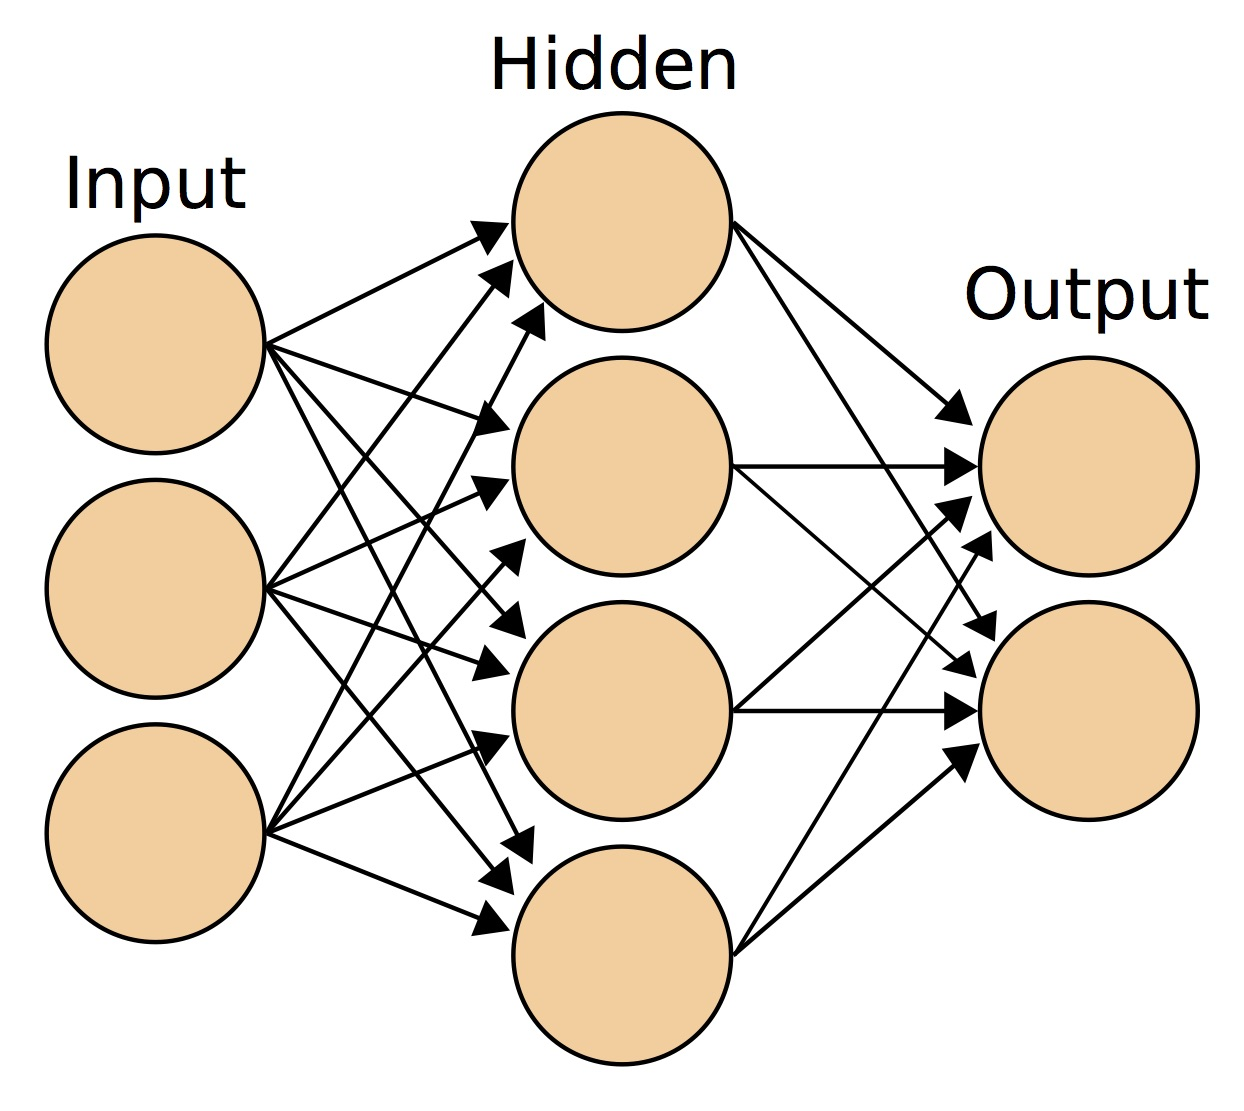
\includegraphics[width=0.4\textwidth]{ann.jpg}
		\vspace{-20pt}
	\end{center}
\end{wrapfigure}

En este trabajo práctico, se analiza el funcionamiento del modelo predictivo
computacional conocido como Redes Neuronales Artificiales (ANNs). Una red
neuronal artificial consta de un grupo interconectado de nodos, similar a la
vasta red de neuronas presente en un cerebro biológico, junto con un gran
número de interconexiones entre nodos, cada una de las cuales posee un peso
sináptico obtenido a partir de algún proceso de entrenamiento que minimice el
error de predicción. Algunos de los aspectos que analizamos en este trabajo son
la dependencia de los valores de entrenamiento, la arquitectura de la red, y el
método de regularización vs. el error en la predicción obtenido. Además se
compara la precisión entre redes neuronales y árboles de decisión para dos
problemas de clasificación particulares.

\pagebreak

%------------------------------------------------

\section*{Apartado a.}  \textbf{Mínimos locales:}
\textit{Baje el dataset dos-elipses de la página de datasets. Cree el archivo
.net necesario. Realice varios entrenamientos con los siguientes parámetros: 6
neuronas en la capa intermedia, 500 patrones en el training set, de los cuales
400 se usan para entrenar y 100 para validar el modelo, 2000 patrones en el
test set, 40000 épocas de entrenamiento, grabando resultados cada 200 o 400
épocas. Pruebe distintos valores de momentum y learning-rate (valores usuales
son 0, 0.5, 0.9 para el momentum y 0.1, 0.01, 0.001 para el learning-rate, pero
no hay por qué limitarse a esos valores), para tratar de encontrar el mejor
mínimo posible de la función error. Con los parámetros dados, hay seguro
soluciones entre 5\% y 6\% de error en test, y tal vez mejores. Confeccione una
tabla con los valores usados para los parámetros y el resultado en test
obtenido. Haga una gráfica de mse de train, validación y test en función del
número de épocas para los valores seleccionados.}\\

\vspace{20pt}

\begin{wrapfigure}{o}{0.45\textwidth}
	\begin{center}
		\vspace{-20pt}
        \includegraphics[width=0.4\textwidth]{{dos_elipses.test}.png}
		\vspace{-20pt}
	\end{center}
\end{wrapfigure}

Con el fin de obtener una mejor intuición de cómo se comporta el error de
clasificación respecto del Learning Rate y el Momentum elegido para el problema
de las dos elipses (derecha), se recolectaron resultados utilizando una escala
logarítmica de 21 valores entre 0.1 y 0.001 para el Learning Rate, mientras que
se usaron 20 valores entre 0 y 0.95 con pasos de 0.05 para el caso del
Momentum. Todos las combinaciones fueron ejecutadas 20 veces y luego se eligió
el valor medio obtenido de ellas en cada caso. Una vez recolectados estos
datos, se realizó un mapa de calor de la superficie de error de clasificación
discreto para estas 420 posibles combinaciones, la misma se muestra a
continuación de manera suavizada (la tabla detallada de los valores se presenta
al final del trabajo). Se encontró que usando un Learning Rate de 0.0063 y
Momentum de 0.85 se consigue el menor error discreto de clasificación, de
aproximadamente un 3\%. Para ésta configuración se incluye una gráfica del MSE
en Entrenamiento, Validación y Test vs. el número de épocas de entrenamiento.
La misma incluye curvas suavizadas para cada tipo de error.

\begin{figure}[H]
\captionsetup[subfigure]{justification=centering, labelformat=empty}
  \centering
  \subfloat[Error discreto de clasificación en función del Momentum y Learning Rate.]
           [Error discreto de clasificación en \\ función del Momentum y Learning Rate.]
            {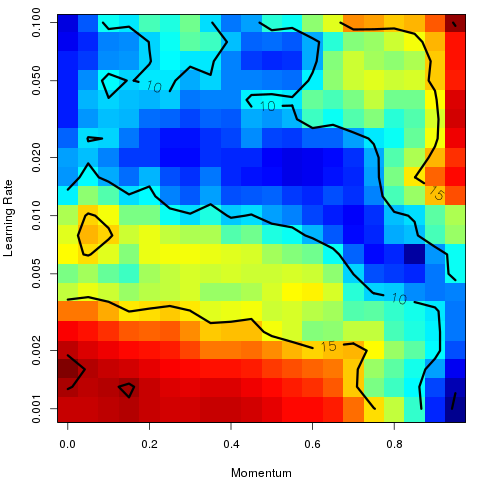
\includegraphics[width=0.5\textwidth]{local_minimums_heatmap.png}}
  \subfloat[MSE en Entrenamiento, Validación y Test para la red de menor error.]
           [MSE en Entrenamiento, Validación\\y Test para la red de menor error.]
            {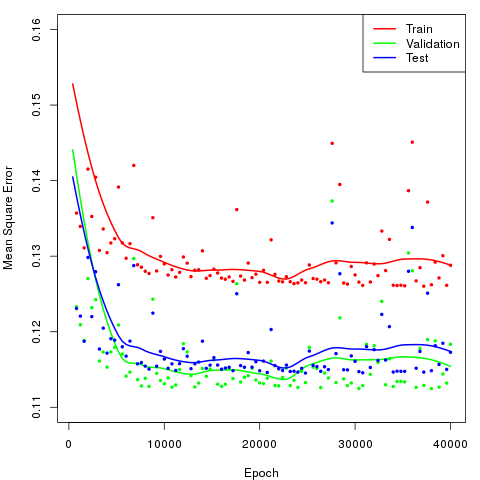
\includegraphics[width=0.5\textwidth]{local_minimums_best_mse.png}}
\end{figure}

Como se puede apreciar en el mapa de calor del error de clasificación, es muy
importante saber elegir correctamente los parámetros de entrenamiento, ya que
hacer un análisis estadístico como el de la figura puede resultar impracticable
en muchos casos. El Learning Rate determina cuánto aprende la red con cada
nueva entrada, mientras que el Momentum le permite al algoritmo "escapar"
de los mínimos locales debidos (posiblemente) al ruido que puede encontrarse en
los datos de entrenamiento. Para este caso en particular, se puede ver que los
mejores resultados se obtienen con valores inversamente proporcionales entre
Momentum y Learning Rate, aunque haría falta un análisis más comprehensivo del
problema para tener una certeza de en qué proporción debe moverse cada
parámetro respecto del otro.

Si en cambio observamos cada tipo de error medio para el entrenamiento que
obtuvo los mejores resultados, puede verse que la red llega al menor error en
alrededor de 23k épocas de entrenamiento. A partir de ahí comienza lentamente a
sobreajustarse a los datos de entrenamiento.

% latex table generated in R 3.3.3 by xtable 1.8-2 package
% Wed May 24 23:47:08 2017
\begin{sidewaystable}[ht]
\centering
\resizebox{\columnwidth}{!}{%
\begin{tabular}{crrrrrrrrrrrrrrrrrrrrr}
\theadfont\diagbox[width=11em]{Momentum}{Learing Rate} & 0.001 & 0.0013 & 0.0016 & 0.002 & 0.0025 & 0.0032 & 0.004 & 0.005 & 0.0063 & 0.0079 & 0.01 & 0.0126 & 0.0158 & 0.02 & 0.0251 & 0.0316 & 0.0398 & 0.0501 & 0.0631 & 0.0794 & 0.1 \\ \hline
     0 & 19.05 & 19.50 & 24.35 & 19.10 & 19.35 & 19.25 & 11.05 & 7.15 & 19.50 & 10.50 & 16.15 & 5.20 & 4.75 & 13.45 & 4.90 & 5.05 & 4.40 & 5.95 & 8.90 & 5.50 & 4.90 \\ 
       0.05 & 19.30 & 19.30 & 19.30 & 18.80 & 18.60 & 17.80 & 14.85 & 13.30 & 17.00 & 19.45 & 19.10 & 17.00 & 17.20 & 5.25 & 17.35 & 5.85 & 19.40 & 4.80 & 5.25 & 5.85 & 6.20 \\ \hline 
         0.1 & 19.55 & 19.65 & 19.50 & 19.35 & 19.50 & 16.50 & 16.35 & 4.70 & 19.10 & 16.50 & 18.35 & 14.45 & 4.50 & 5.20 & 17.80 & 6.25 & 4.40 & 24.35 & 6.10 & 5.25 & 19.65 \\ 
           0.15 & 19.65 & 24.35 & 18.35 & 18.60 & 19.00 & 10.40 & 14.30 & 5.00 & 5.85 & 15.60 & 10.20 & 4.55 & 3.85 & 5.10 & 4.95 & 16.35 & 10.90 & 5.30 & 8.20 & 7.95 & 5.15 \\ \hline 
             0.2 & 19.40 & 19.50 & 18.55 & 18.85 & 16.80 & 16.15 & 11.25 & 16.30 & 18.00 & 17.45 & 15.95 & 13.00 & 19.05 & 5.20 & 7.35 & 5.85 & 4.65 & 15.50 & 9.00 & 6.05 & 19.70 \\ 
               0.25 & 19.30 & 19.25 & 18.35 & 19.45 & 19.35 & 17.10 & 10.35 & 10.55 & 17.45 & 14.60 & 7.30 & 5.45 & 6.65 & 4.60 & 4.30 & 7.65 & 19.40 & 8.05 & 15.55 & 9.40 & 4.65 \\ \hline 
                 0.3 & 19.45 & 19.10 & 18.65 & 17.60 & 17.35 & 13.40 & 18.05 & 14.65 & 14.90 & 17.10 & 4.55 & 4.40 & 4.35 & 5.35 & 7.70 & 5.60 & 4.70 & 5.75 & 5.55 & 16.65 & 19.75 \\ 
                   0.35 & 19.45 & 19.50 & 19.55 & 15.10 & 13.85 & 14.85 & 6.90 & 13.90 & 14.00 & 17.50 & 17.15 & 10.10 & 16.05 & 6.60 & 4.80 & 14.65 & 4.75 & 19.40 & 8.50 & 19.25 & 5.15 \\ \hline 
                     0.4 & 20.20 & 19.70 & 18.90 & 16.05 & 15.50 & 14.15 & 10.80 & 17.10 & 19.10 & 4.35 & 5.20 & 5.15 & 4.20 & 7.85 & 5.25 & 4.50 & 5.75 & 6.00 & 6.10 & 14.50 & 4.70 \\ 
                       0.45 & 19.55 & 18.70 & 19.65 & 17.40 & 17.90 & 19.40 & 7.10 & 13.15 & 16.05 & 18.15 & 14.95 & 5.10 & 5.30 & 4.60 & 19.40 & 6.85 & 19.50 & 6.40 & 6.40 & 4.20 & 7.95 \\ \hline 
                         0.5 & 19.50 & 18.90 & 17.70 & 18.10 & 11.00 & 9.15 & 17.40 & 13.35 & 15.40 & 6.25 & 4.10 & 14.75 & 4.70 & 5.60 & 3.80 & 6.20 & 19.45 & 6.40 & 4.10 & 6.70 & 19.40 \\ 
                           0.55 & 17.85 & 19.35 & 17.75 & 14.95 & 16.00 & 14.00 & 17.00 & 13.85 & 11.30 & 15.30 & 9.50 & 5.60 & 5.00 & 5.30 & 7.45 & 6.40 & 5.75 & 6.30 & 5.85 & 4.45 & 7.10 \\ \hline 
                             0.6 & 19.25 & 18.25 & 17.65 & 17.30 & 3.40 & 13.50 & 18.95 & 12.85 & 16.75 & 7.45 & 6.35 & 5.10 & 5.95 & 5.15 & 3.70 & 24.35 & 24.35 & 4.35 & 5.00 & 4.55 & 19.70 \\ 
                               0.65 & 19.55 & 17.75 & 17.00 & 19.15 & 6.10 & 16.15 & 19.25 & 15.10 & 14.85 & 4.05 & 4.10 & 16.25 & 5.30 & 5.25 & 7.80 & 5.70 & 4.65 & 19.10 & 21.20 & 4.75 & 12.80 \\ \hline 
                                 0.7 & 18.35 & 15.70 & 18.50 & 19.25 & 15.60 & 4.30 & 10.85 & 11.50 & 5.15 & 4.80 & 4.65 & 5.85 & 5.00 & 4.50 & 7.25 & 19.25 & 6.60 & 14.85 & 19.90 & 4.75 & 24.35 \\ 
                                   0.75 & 17.20 & 5.80 & 5.30 & 19.35 & 19.35 & 16.60 & 5.10 & 4.45 & 4.35 & 4.75 & 5.20 & 6.90 & 7.70 & 7.55 & 8.60 & 19.25 & 19.50 & 14.60 & 13.20 & 5.20 & 19.30 \\ \hline 
                                     0.8 & 16.65 & 4.35 & 18.15 & 13.20 & 5.05 & 10.70 & 16.95 & 5.35 & 3.45 & 19.45 & 7.55 & 19.45 & 11.70 & 19.25 & 5.85 & 5.25 & 10.65 & 19.05 & 5.45 & 19.25 & 14.20 \\ 
                                       0.85 & 14.00 & 16.60 & 4.40 & 17.65 & 7.75 & 16.35 & 4.50 & 5.45 & 3.00 & 8.50 & 5.00 & 7.75 & 24.35 & 5.65 & 14.05 & 14.65 & 4.05 & 19.70 & 7.15 & 15.55 & 15.80 \\ \hline 
                                         0.9 & 4.35 & 4.85 & 12.50 & 15.55 & 9.60 & 17.10 & 5.50 & 5.20 & 5.85 & 19.35 & 8.05 & 19.45 & 19.60 & 19.55 & 7.60 & 6.20 & 12.65 & 15.15 & 15.25 & 12.10 & 15.75 \\ 
                                           0.95 & 3.00 & 3.60 & 4.20 & 5.70 & 9.40 & 5.45 & 5.10 & 19.45 & 5.80 & 19.00 & 6.30 & 24.35 & 20.00 & 14.75 & 24.35 & 24.35 & 24.35 & 16.30 & 22.40 & 16.80 & 24.35 \\ 
\hline
\end{tabular}
}
\end{sidewaystable}



%------------------------------------------------

\section*{Apartado b.} \textbf{Arquitectura:} \textit{Entrene redes neuronales
para resolver el problema de clasificación de las espirales anidadas. Use un
número creciente de neuronas en la capa intermedia: 2, 5, 10, 20, 40. Valores
posibles para los demás parámetros de entrenamiento: learning rate 0.01,
momentum 0.5, 1600 datos para ajustar los modelos, 400 para validar, 2000 para
testear, 40000 épocas de entrenamiento, grabando cada 400. Para cada uno de los
cinco modelos obtenidos, graficar en el plano xy las clasificaciones sobre el
conjunto de test (para 10 neuronas hay solución con error del orden de 22\%,
para 40 del orden de 10\%, el tiempo de ejecución puede llegar a 20
minutos).}\\

Para analizar como afecta la cantidad de neuronas en la capa intermedia de una
red neuronal encargada de resolver el problema de las espirales anidadas, se
entrenaron distintas redes con 2, 5, 10, 20 y 40 neuronas en dicha capa. Los
resultados muestran el valor medio de 20 ejecuciones en cada caso. A
continuación se incluyen gráficas con las predicciones para cada caso, junto
con el conjunto de prueba utilizado.

\begin{figure}[H]
\captionsetup[subfigure]{justification=centering, labelformat=empty}
  \centering
  %\caption*yy{\textbf{Entrenamiento con n=150.}}
  \subfloat[][\phantom{aaa}\textbf{N = 2}]
    {\includegraphics[width=0.5\textwidth]{{spiral.1.2.predic.d}.png}}
  \subfloat[][\phantom{aaa}\textbf{N = 5}]
    {\includegraphics[width=0.5\textwidth]{{spiral.1.5.predic.d}.png}}
\end{figure}

\begin{figure}[H]
\captionsetup[subfigure]{justification=centering, labelformat=empty}
  \centering
  %\caption*{\textbf{Entrenamiento con n=150.}}
  \subfloat[][\phantom{aaa}\textbf{N = 10}]
    {\includegraphics[width=0.5\textwidth]{{spiral.1.10.predic.d}.png}}
  \subfloat[][\phantom{aaa}\textbf{N = 20}]
    {\includegraphics[width=0.5\textwidth]{{spiral.1.20.predic.d}.png}}
\end{figure}

\begin{figure}[H]
\captionsetup[subfigure]{justification=centering, labelformat=empty}
  \centering
  %\caption*{\textbf{Entrenamiento con n=150.}}
  \subfloat[][\phantom{aaa}\textbf{N = 40}]
    {\includegraphics[width=0.5\textwidth]{{spiral.1.40.predic.d}.png}}
  \subfloat[][\phantom{aaa}\textbf{Test}]
    {\includegraphics[width=0.5\textwidth]{{spiral.test}.png}}
\end{figure}

\begin{wrapfigure}{o}{0.45\textwidth}
	\begin{center}
		\vspace{-20pt}
        \includegraphics[width=0.4\textwidth]{{spiral_error}.png}
		\vspace{-20pt}
	\end{center}
\end{wrapfigure}

Se puede apreciar claramente que una mayor cantidad de neuronas mejora
considerablemente la precisión de la red neuronal resultante, a costa por
supuesto de un mayor tiempo de entrenamiento, debido a la gran cantidad de
conexiones nuevas que deben ajustarse para cada nueva neurona que se agrega a
la red. Sin embargo, parece existir un número de neuronas para el cual seguir
agrandando el tamaño la red no tiene sentido, ya que no se obtienen mejorías
substanciales en la precisión de la misma. Para nuestro ejemplo en particular,
este valor parece estar entre 20 y 40 neuronas para la capa intermedia, como se
muestra en la figura de la derecha.

%------------------------------------------------

\section*{Apartado c.} \textbf{Regularización} \textit{Baje el dataset Ikeda de
la página de datasets. Realice entrenamientos usando el 95\% del archivo .data
para entrenar, y el resto para validar (todos los otros parámetros hay que
mantenerlos como están en el archivo .net original que viene con el dataset).
Realice otros entrenamientos cambiando la relación a 75\%-25\%, y a 50\%-50\%.
En cada caso seleccione un resultado que considere adecuado, y genere gráficas
del mse en train, validación y test.}\\

Otro aspecto importante a la hora de entrenar una red neuronal resulta ser la
proporción de datos usados entre entrenamiento y validación. Para realizar un
análisis de este parámetro se utilizó el dataset \textit{ikeda}, donde se
entrenaron tres conjuntos de redes, con ratios de entrenamiento/validación de
50/50, 75/25 y 95/5 en cada caso. Luego se tomó nuevamente aquella red de valor
medio del error para cada conjunto. Los errores medios de entrenamiento,
validación y prueba para cada conjunto se pueden observar en las siguientes
gráficas.

\begin{figure}[H]
\captionsetup[subfigure]{justification=centering, labelformat=empty}
  \centering
  \subfloat[][\phantom{aaaa}\textbf{50/50}]
    {\includegraphics[width=0.5\textwidth]{{ikeda.50.mse.avg}.png}}
  \subfloat[][\phantom{aaaa}\textbf{75/25}]
    {\includegraphics[width=0.5\textwidth]{{ikeda.75.mse.avg}.png}}
\end{figure}

\begin{figure}[H]
\captionsetup[subfigure]{justification=centering, labelformat=empty}
  \centering
  \subfloat[][\phantom{aaaa}\textbf{95/5}]
    {\includegraphics[width=0.5\textwidth]{{ikeda.95.mse.avg}.png}}
\end{figure}

Lo primero que se observa es el error mínimo de prueba obtenido con cada
configuración de la red, el cual resulta de alrededor del 13\% para el caso del
ratio 50/50, mientras que para los ratios de 75/25 y 95/5 estos resultan de
alrededor de 7\% y 8\% para cada uno respectivamente. Esto pondría en evidencia
que usar una cantidad reducida de datos para el conjunto de entrenamiento
produce inevitablemente un resultado final bastante pobre, ya que para el caso
del ratio 50/50 solo se usaron 50 valores para entrenar la red. 

Otro dato interesante que puede extraerse de los gráficos es el grado de
sobreajuste que la red adquiere dependiendo del ratio de
entrenamiento/validación usado. Para el caso del ratio 50/50, la red tiende a 
sobreajustarse rápidamente, consiguiendo el mínimo error de prueba en alrededor
de 5k épocas de entrenamiento. Si analizamos ahora los ratios de 75/25 y 95/5
este sobreajuste se produce mucho más lentamente a medida que se usan más datos
para entrenar y menos para validar, obteniendo además el mínimo error de prueba
en alrededor de 3k épocas de entrenamiento para ambos casos. Cabe destacar que
una cantidad muy pequeña de datos de validación conduce a un error de
validación más errático respecto de la cantidad de épocas de entrenamiento, ya
que entre más pequeño sea este conjunto, si alguno de sus valores posee ruido,
el mismo afecta en mayor proporción al error de validación.

%------------------------------------------------

\section*{Apartado d.} \textbf{Regularización:} \textit{Modifique el programa
bp.c para implementar otro método de regularización, el weight-decay. Agregue
un término de penalización a la magnitud de los pesos en la función error, y la
modificación necesaria a su derivada. El parámetro gamma hay que agregarlo al
archivo de configuración. En lugar del error sobre el conjunto de validación,
en este caso es interesante analizar curvas del error de ajuste, del término de
penalización y del error en test en función del número de épocas.  Una vez
implementado, aplíquelo al dataset Sunspots. Busque el valor de gamma adecuado
para conseguir un equilibrio entre evitar el sobreajuste y hacer el modelo
demasiado rígido. En este caso todos los registros del archivo .data se deben
usar para el entrenamiento, ya que la regularización se realiza con la
penalización a los pesos grandes. Todos los otros parámetros se deben dejar
como en el archivo .net que viene con el dataset. Entregue el programa
modificado, y curvas de los tres errores para el valor de gamma elegido, y para
algún otro valor en que haya observado sobreajuste.}\\

Para este apartado, se modificó el programa \textit{bp} para implementar el
método de regularización conocido como \textit{weight-decay} el cual decrementa
los pesos de las conexiones sinápticas en cada iteración por un pequeño factor
de penalización que depende del parámetro externo $\gamma$ (gamma), con el fin
de evitar el sobreajuste de la red. Para analizar como el valor $\gamma$
repercute en el entrenamiento de la red, se entrenaron conjuntos de 20 redes
para los valores $10^i$ con $i$ entre -8 y 0. Para cada conjunto se tomó aquel
de error medio. Los siguientes pares de gráficas muestran el error medio
cuadrático de entrenamiento y prueba, junto con el factor de penalización en
el ajuste de los pesos en cada época (decay). 

\begin{figure}[H]
\captionsetup[subfigure]{justification=centering, labelformat=empty}
  \centering
  \caption*{\textbf{$\gamma$ = 1}}
  \vspace{-20pt}
  \subfloat[][]{\includegraphics[width=0.4\textwidth]{{ssp.1.mse.avg.error}.png}}
  \subfloat[][]{\includegraphics[width=0.4\textwidth]{{ssp.1.mse.avg.decay}.png}}
\end{figure}

\begin{figure}[H]
\captionsetup[subfigure]{justification=centering, labelformat=empty}
  \centering
  \caption*{\textbf{$\gamma$ = 0.1}}
  \vspace{-20pt}
  \subfloat[][]{\includegraphics[width=0.4\textwidth]{{ssp.0.1.mse.avg.error}.png}}
  \subfloat[][]{\includegraphics[width=0.4\textwidth]{{ssp.0.1.mse.avg.decay}.png}}
\end{figure}

\begin{figure}[H]
\captionsetup[subfigure]{justification=centering, labelformat=empty}
  \centering
  \caption*{\textbf{$\gamma$ = 0.01}}
  \vspace{-20pt}
  \subfloat[][]{\includegraphics[width=0.4\textwidth]{{ssp.0.01.mse.avg.error}.png}}
  \subfloat[][]{\includegraphics[width=0.4\textwidth]{{ssp.0.01.mse.avg.decay}.png}}
\end{figure}

\begin{figure}[H]
\captionsetup[subfigure]{justification=centering, labelformat=empty}
  \centering
  \caption*{\textbf{$\gamma$ = 0.001}}
  \vspace{-20pt}
  \subfloat[][]{\includegraphics[width=0.4\textwidth]{{ssp.0.001.mse.avg.error}.png}}
  \subfloat[][]{\includegraphics[width=0.4\textwidth]{{ssp.0.001.mse.avg.decay}.png}}
\end{figure}

\begin{figure}[H]
\captionsetup[subfigure]{justification=centering, labelformat=empty}
  \centering
  \caption*{\textbf{$\gamma$ = 0.0001}}
  \vspace{-20pt}
  \subfloat[][]{\includegraphics[width=0.4\textwidth]{{ssp.0.0001.mse.avg.error}.png}}
  \subfloat[][]{\includegraphics[width=0.4\textwidth]{{ssp.0.0001.mse.avg.decay}.png}}
\end{figure}

\begin{figure}[H]
\captionsetup[subfigure]{justification=centering, labelformat=empty}
  \centering
  \caption*{\textbf{$\gamma$ = 0.00001}}
  \vspace{-20pt}
  \subfloat[][]{\includegraphics[width=0.4\textwidth]{{ssp.0.00001.mse.avg.error}.png}}
  \subfloat[][]{\includegraphics[width=0.4\textwidth]{{ssp.0.00001.mse.avg.decay}.png}}
\end{figure}

\begin{figure}[H]
\captionsetup[subfigure]{justification=centering, labelformat=empty}
  \centering
  \caption*{\textbf{$\gamma$ = 0.000001}}
  \vspace{-20pt}
  \subfloat[][]{\includegraphics[width=0.4\textwidth]{{ssp.0.000001.mse.avg.error}.png}}
  \subfloat[][]{\includegraphics[width=0.4\textwidth]{{ssp.0.000001.mse.avg.decay}.png}}
\end{figure}

\begin{figure}[H]
\captionsetup[subfigure]{justification=centering, labelformat=empty}
  \centering
  \caption*{\textbf{$\gamma$ = 0.0000001}}
  \vspace{-20pt}
  \subfloat[][]{\includegraphics[width=0.4\textwidth]{{ssp.0.0000001.mse.avg.error}.png}}
  \subfloat[][]{\includegraphics[width=0.4\textwidth]{{ssp.0.0000001.mse.avg.decay}.png}}
\end{figure}

\begin{figure}[H]
\captionsetup[subfigure]{justification=centering, labelformat=empty}
  \centering
  \caption*{\textbf{$\gamma$ = 0.00000001}}
  \vspace{-20pt}
  \subfloat[][]{\includegraphics[width=0.4\textwidth]{{ssp.0.00000001.mse.avg.error}.png}}
  \subfloat[][]{\includegraphics[width=0.4\textwidth]{{ssp.0.00000001.mse.avg.decay}.png}}
\end{figure}

\begin{wrapfigure}{o}{0.45\textwidth}
	\begin{center}
		\vspace{-20pt}
        \includegraphics[width=0.4\textwidth]{{sunspots_error}.png}
		\vspace{-20pt}
	\end{center}
\end{wrapfigure}

En las gráficas se aprecia que los valores muy grandes de $\gamma$ penalizan
demasiado el entrenamiento, haciéndola rígida y evitando el aprendizaje. Si en
cambio analizamos los valores de $\gamma$ muy pequeños, se puede notar que su
efecto en la red es prácticamente despreciable, y ya que la red no utiliza
datos de validación, se vuelve inevitable el sobreajuste.

Si se observa el gráfico de error cuadratico medio vs. $\gamma$ de la derecha
se aprecia que el mejor resultado se encuentra en un punto medio entre los
valores extremos de $\gamma$. Puntualmente, el valor más adecuado de
penalización resulta ser $\gamma = 0.00001$, minimizando el error final de la
red sin que esta se vuelva demasiado rígida.

%------------------------------------------------

\section*{Apartado e.} \textbf{Dimensionalidad: } \textit{Repita el punto 7 del
Práctico 1, usando redes con 6 unidades en la capa intermedia. Genere una
gráfica con los resultados de redes y árboles.}\\

En este apartado se analiza la dependencia entre el error de test discreto vs.
la dimensionalidad del problema, comparando la precisión obtenida utilizando
Árboles de Decisión y Redes Neuronales. En particular, se compara como se
comportan ambos modelos para el caso de los problemas \textit{diagonal} y
\textit{paralelo}. La siguiente gráfica muestra los resultados obtenidos en el
práctico anterior para ambos problemas usando Árboles de Decisión, junto con
los datos obtenidos al entrenar redes neuronales para los mismos datasets.


\begin{figure}[H]
\captionsetup[subfigure]{justification=centering, labelformat=empty}
  \centering
  \subfloat[][Error discreto vs. Dimensionalidad para los problemas
      \textit{diagonal} y \textit{paralelo}
          utilizando Árboles de Decisión (DT) y Redes Neuronales Artificiales
          (ANN).]{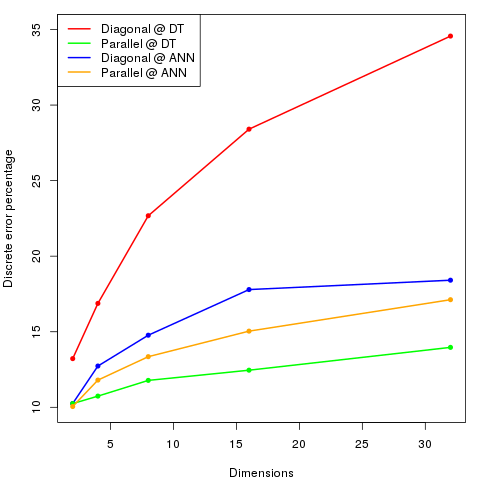
\includegraphics[width=0.7\textwidth]{anns_vs_dtree.png}}
\end{figure}

Lo primero que se aprecia es que ambos métodos de clasificación se ven
afectados negativamente por el aumento en la dimensionalidad del problema. Sin
embargo, en el caso de las Redes Neuronales, éstas se ven menos afectadas por
la complejidad del mismo, y tienden a resultar en valores de error de test
similares para ambos problemas. Mientras que para los Árboles de Decisión, la
dimensionalidad repercute de manera muy diferente para distintos tipos de
problemas. En nuestro caso, es interesante notar que las curvas de los
problemas \textit{paralelo} y \textit{diagonal} entrenados usando Árboles de
Decisión acotan inferior y superiormente a sus homólogas entrenadas mediante
Redes Neuronales respectivamente.

\end{document}
